\documentclass[12pt]{article}
\usepackage[margin=0.75in]{geometry}
\usepackage{graphicx}
\usepackage{float}
\setlength{\parindent}{0mm}

\begin{document}

{\centering
\large Class 16 Activity \par
}
\hfill \break \vspace{-4mm}

1. A car starts from rest and accelerates uniformly with no slipping between the tires and road.
If one of the wheels has an angular acceleration of 2.8 $rad/s^2$ and it takes 8 seconds for the car to reach a speed of 9 m/s, what is the radius of the wheel?
\hfill \break

2. The figure below shows an aerial view of a door that can rotate frictionlessly about its hinge.
Two forces are applied as shown, one halfway down the length of the door and the other one at the very end of the door.
If the length of the door is 1.8 m and its mass is 25 kg, calculate the magnitude and direction (clockwise or counterclockwise) of the agular acceleration.
%
\begin{figure}[H]
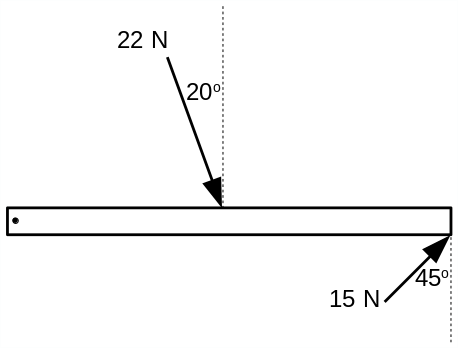
\includegraphics[scale=0.50]{figures/torque-rod.png}
\end{figure}

3. A satellite circles a planet every 2.8 h in an orbit having a radius of $1.2 \times 10^7$ m.
If the radius of the planet is $5.0 \times 10^6$ m, what is the magnitude of the free-fall acceleration on its surface?
\hfill \break

4. A massless disk is nailed to a wall through its center.
The disk can rotate frictionlessly about the nail. 
Three masses are glued to the disk as shown.
A rope is wrapped around the disk several times and then attached to a 34 kg hanging mass.
Calculate the angular acceleration of the disk.
%
\begin{figure}[H]
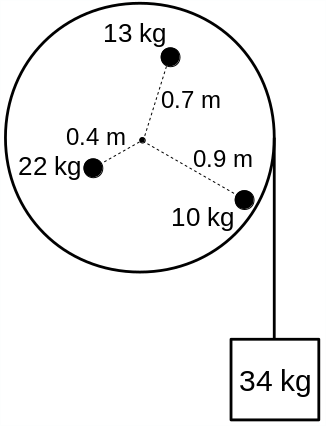
\includegraphics[scale=0.50]{figures/mass-hanging-from-disk.png}
\end{figure}

5. A mass of 10 kg is attached to a spring and set into simple harmonic motion.
If it takes 7 s to complete 3 full oscillations, what is the value of the spring constant?
\hfill \break

6. 
\begin{figure}[H]
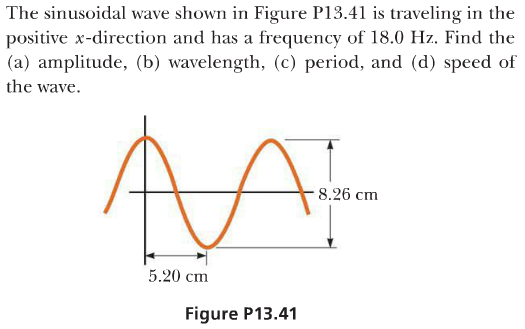
\includegraphics[scale=0.70]{figures/sine-wave.png}
\end{figure}


\end{document}
